\documentclass[11pt,letter]{article}
% \include{macro-file}

\def\mainroot{ell_1}

%%%%%% Margins and spacing
\usepackage[top=1in, bottom=1in, left=1in, right=1in]{geometry}
\usepackage{algorithm}
\usepackage{amsmath}
\usepackage{url}
\usepackage{caption}
\usepackage[compact]{titlesec}
%\usepackage{bm}
\usepackage{txfonts} %\usepackage{times}
\usepackage{color}
\usepackage{tikz}
\usetikzlibrary{calc}
\usepackage{cancel}
\usepackage{soul}
\usepackage{graphicx}
\usepackage{caption}
\usepackage{subcaption}
\usepackage{algpseudocode}

\usepackage{sidecap}
\sidecaptionvpos{figure}{c}

\usepackage{enumitem}
\setlist{nolistsep}

%\setcounter{MaxMatrixCols}{20}

\newcommand\mjsnote[1]{{\bf [#1 -mjs]}}

\newcommand{\meas}{{\mathbf \mu}}
\newcommand{\tightpgh}[1]{\vskip 3pt\noindent\textbf{#1}}
\newcommand{\signalw}{{\mathbf w}}
\newcommand{\signalx}{{\mathbf x}}
\newcommand{\signaly}{{\mathbf y}}
\newcommand{\signalz}{{\mathbf z}}

%\expandafter\def\expandafter\normalsize\expandafter{%
%    \normalsize
%    \setlength\abovedisplayskip{2pt}
%    \setlength\belowdisplayskip{2pt}
%    \setlength\abovedisplayshortskip{0pt}
%    \setlength\belowdisplayshortskip{0pt}
%}\makeatother
%
%\renewcommand\floatpagefraction{.9}
%\renewcommand\topfraction{.9}
%\renewcommand\bottomfraction{.9}
%\renewcommand\textfraction{.1}   
%\setlength{\textfloatsep}{10pt plus 1.0pt minus 2.0pt}

% Jian \DeclareMathOperator*{\median}{median}
\newcommand{\mb}{\ensuremath\mathbf}
\newcommand{\F}{\ensuremath\mathbb{F}}

\title{UI for RNA-seq quantification \footnote{Course Project Report of CSE 549.}}
\author{
%\alignauthor
Yigong Wang\\
       {\small SBU ID: 109973706}\\
       {\small Department of Computer Science}\\
       {\small Stony Brook University} \\
       {\small \texttt{yigwang@cs.stonybrook.edu}}
%\alignauthor
\and
Hongjin Zhu \\
       {\small SBU ID: 109748818}\\
       {\small Department of Computer Science}\\
       {\small Stony Brook University} \\
       {\small \texttt{hozzhu@cs.stonybrook.edu}}
%\alignauthor
\and
Jianglin Wu \\
       {\small SBU ID: 108075432}\\
       {\small Department of Computer Science}\\
       {\small Stony Brook University} \\
       {\small \texttt{jiangwu@cs.stonybrook.edu}}
%\alignauthor
\and
%\alignauthor
Jian Yang \\
       {\small SBU ID: 110168771}\\
       {\small Department of Computer Science}\\
       {\small Stony Brook University}\\
       {\small \texttt{yang16@cs.stonybrook.edu}}
}
\date{}


\raggedbottom

\begin{document}
\maketitle

\begin{abstract}
RNA sequencing, is a technology that uses the capabilities of next-generation sequencing to reveal a snapshot of RNA presence and quantity from a genome at a given moment in time. There are many modern algorithms for RNA-seq but there is few visualization about the algorithms' results. Based on this status, we implemented a UI for RNA-Seq quality comparison between various of algorithms. The UI could upload results from algorithms, generate plots and tables for quality metrics and a user could interactively view any data on the plots.
\end{abstract}

\thispagestyle{empty}
\addtocounter{page}{0}

\section {Introduction}

Software developed by programmer can process high throughput RNA-seq data and create detail results for Biologist and Bioinformatician for further analyzing. However, these tools cannot replace the role of a professional user who knows how to deal with the data and the meaning behind the number and text.  A simple graph contains more information than paragraphs of text description.  So, to provide an easy way for Biologist to research on the output data, we have our User Interface which consists of following functionalists: Bar chart for basic statatical information about the data; Scatter Plots for algorithm output data visulization, comparison and analysis; and Metrics for performance evaluation.   \\


\section {UI Architecture}
We implemented this from four components: backend scripts, server, front-end, webpage. \\
\subsection {Backend}
At backend scripts, we did the following jobs.
\begin{enumerate}
\item Calculate the statistics from the transcript. \\
We calculate the data such as GC content, ration of each nucleotides.
\item Load data from result files for algorithms and also the ground truth from profile files according to given parser.
\item Concat the data of results, the ground truth and the statistics based on transcript name as index to a large table.
\item Provide the API to query the data for UI layers.
\item Calculate the performance evaluation matrix.
\end{enumerate}
The API contains the following methods.

\subsection {Frontend}
We used and modified open source bootstrap template SB Admin 2 \cite{sb_admin_2} as our webpage, then integrated and implmented following:\\
\begin{enumerate}
\item Javascript public library:\\
Jquery: jquery-1.8.3.min.js\\
D3js: d3.v3.min.js \cite{d3_scatterplot}\\
\item Javascript library which we implemented:\\
chart.js:  plot all the scatter charts.\\
data.js: using Ajax call to fetch data from server.\\
dropDownList.js: using Ajax call to fetch algorithm and attribute information from server. Change drop down list dynamicly based on user selection.\\
\end{enumerate}

Design detais:
\begin{enumerate}
\item Dynamic drop list.\\
a. Using Ajax call to fetch Json data from user, which contains all feasible algorithms and their relevent attribute.\\
b. Listening to user selection of algorithm, and dynamic change the attributes drop down list.\\
c. Get user's selections from drop down list and send request to server. Then get data to plot scatter charts.\\

\item There are three type of scatter charts.\\
a. Scatter Plot for a Single Algorithm\\
Get user input from front end, send requests through Ajax call to get matched data from server. Get each node and plot them on svg using D3js.\\
Requirement input value from user: {algorithm name, x axis, y axis}\\

b. Scatter Plot for two Algorithms on the same metrics\\
Get user input from front end, send requests through Ajax call to get matched data from server. Get each node and plot them on svg using D3js.\\
Requirement input value from user: {algorithm 1, algorithm 2, a axis, y axis}\\

c. Scatter Plot for two Algorithms on the same feature\\
Get user input from front end, send requests through Ajax call to get matched data from server. Get each node and plot them on svg using D3js.\\
Requirement input value from user: {algorithm 1, algorithm 2, attribute}\\

\item Interacter with user. \\
When user mouse put on the spot from any scatter charts. It will display the name of the node, the x attribute value and y attribute value, and other information that user designed to display. \\

\item Input check.\\
Using Javascript to check user selections' validation. For example, user are not allowed to choose empty content and click the submit button. There will be some alert message.\\

\end{enumerate}

\section {Installation and Usage}

This project provides a web-based user interface, which allows users access it locally or remotely. In this section, we give a brief introduction of installation. \\
The project require following package/software: \\
\begin{enumerate}
\item Modern web browser\\
A modern web browser is required for the user interface. Because the interactive and data visualisation are highly depend on JavaScripts libraries, the latest version browser is highly recommended for better efficiency and experience.\\
\item Python 2.7.9 or later\\
The website framework and data processing are based on Python programming language.\\
\item Django\\
Django provides a basic web server, as well as a web framework. It lays between browser and data. To install Django, using the command (Please note that you might need the administrator privilege, e.g. sudo before pip command):
pip install django\\
\item django-cors-header\\
django-cors-headers library enables cross sites recourse sharing of the server.
pip install django-cors-headers\\
\item pandas, scipy, matplotlib\\
These libraries are used for data processing and bar charts plotting.
pip install pandas scipy matplotlib\\


\end{enumerate}
To run the project, go to ‘server’ folder of the project, use following command: \\
python manage.py runserver 8000 \\
This command will run the server and listen to localhost port 8000. Next, open a browser then navigate to http://127.0.0.1:8000/. \\

\section {UI Features}
We implemented the following features for the quality metrics with interactive modes to compare and view quality about algorithms. Currently we support 3 algorithms and a ground truth is added to compare the precision and the recall ratios.
\subsection {Bar Chart for algorithms}
We support the bar chart for all the algorithms to calculate the number of reads for each algorithm mapped in the experiment. One example is showed in figure \ref{fig:barchart_numreads}.

\begin{figure}
 \centering
 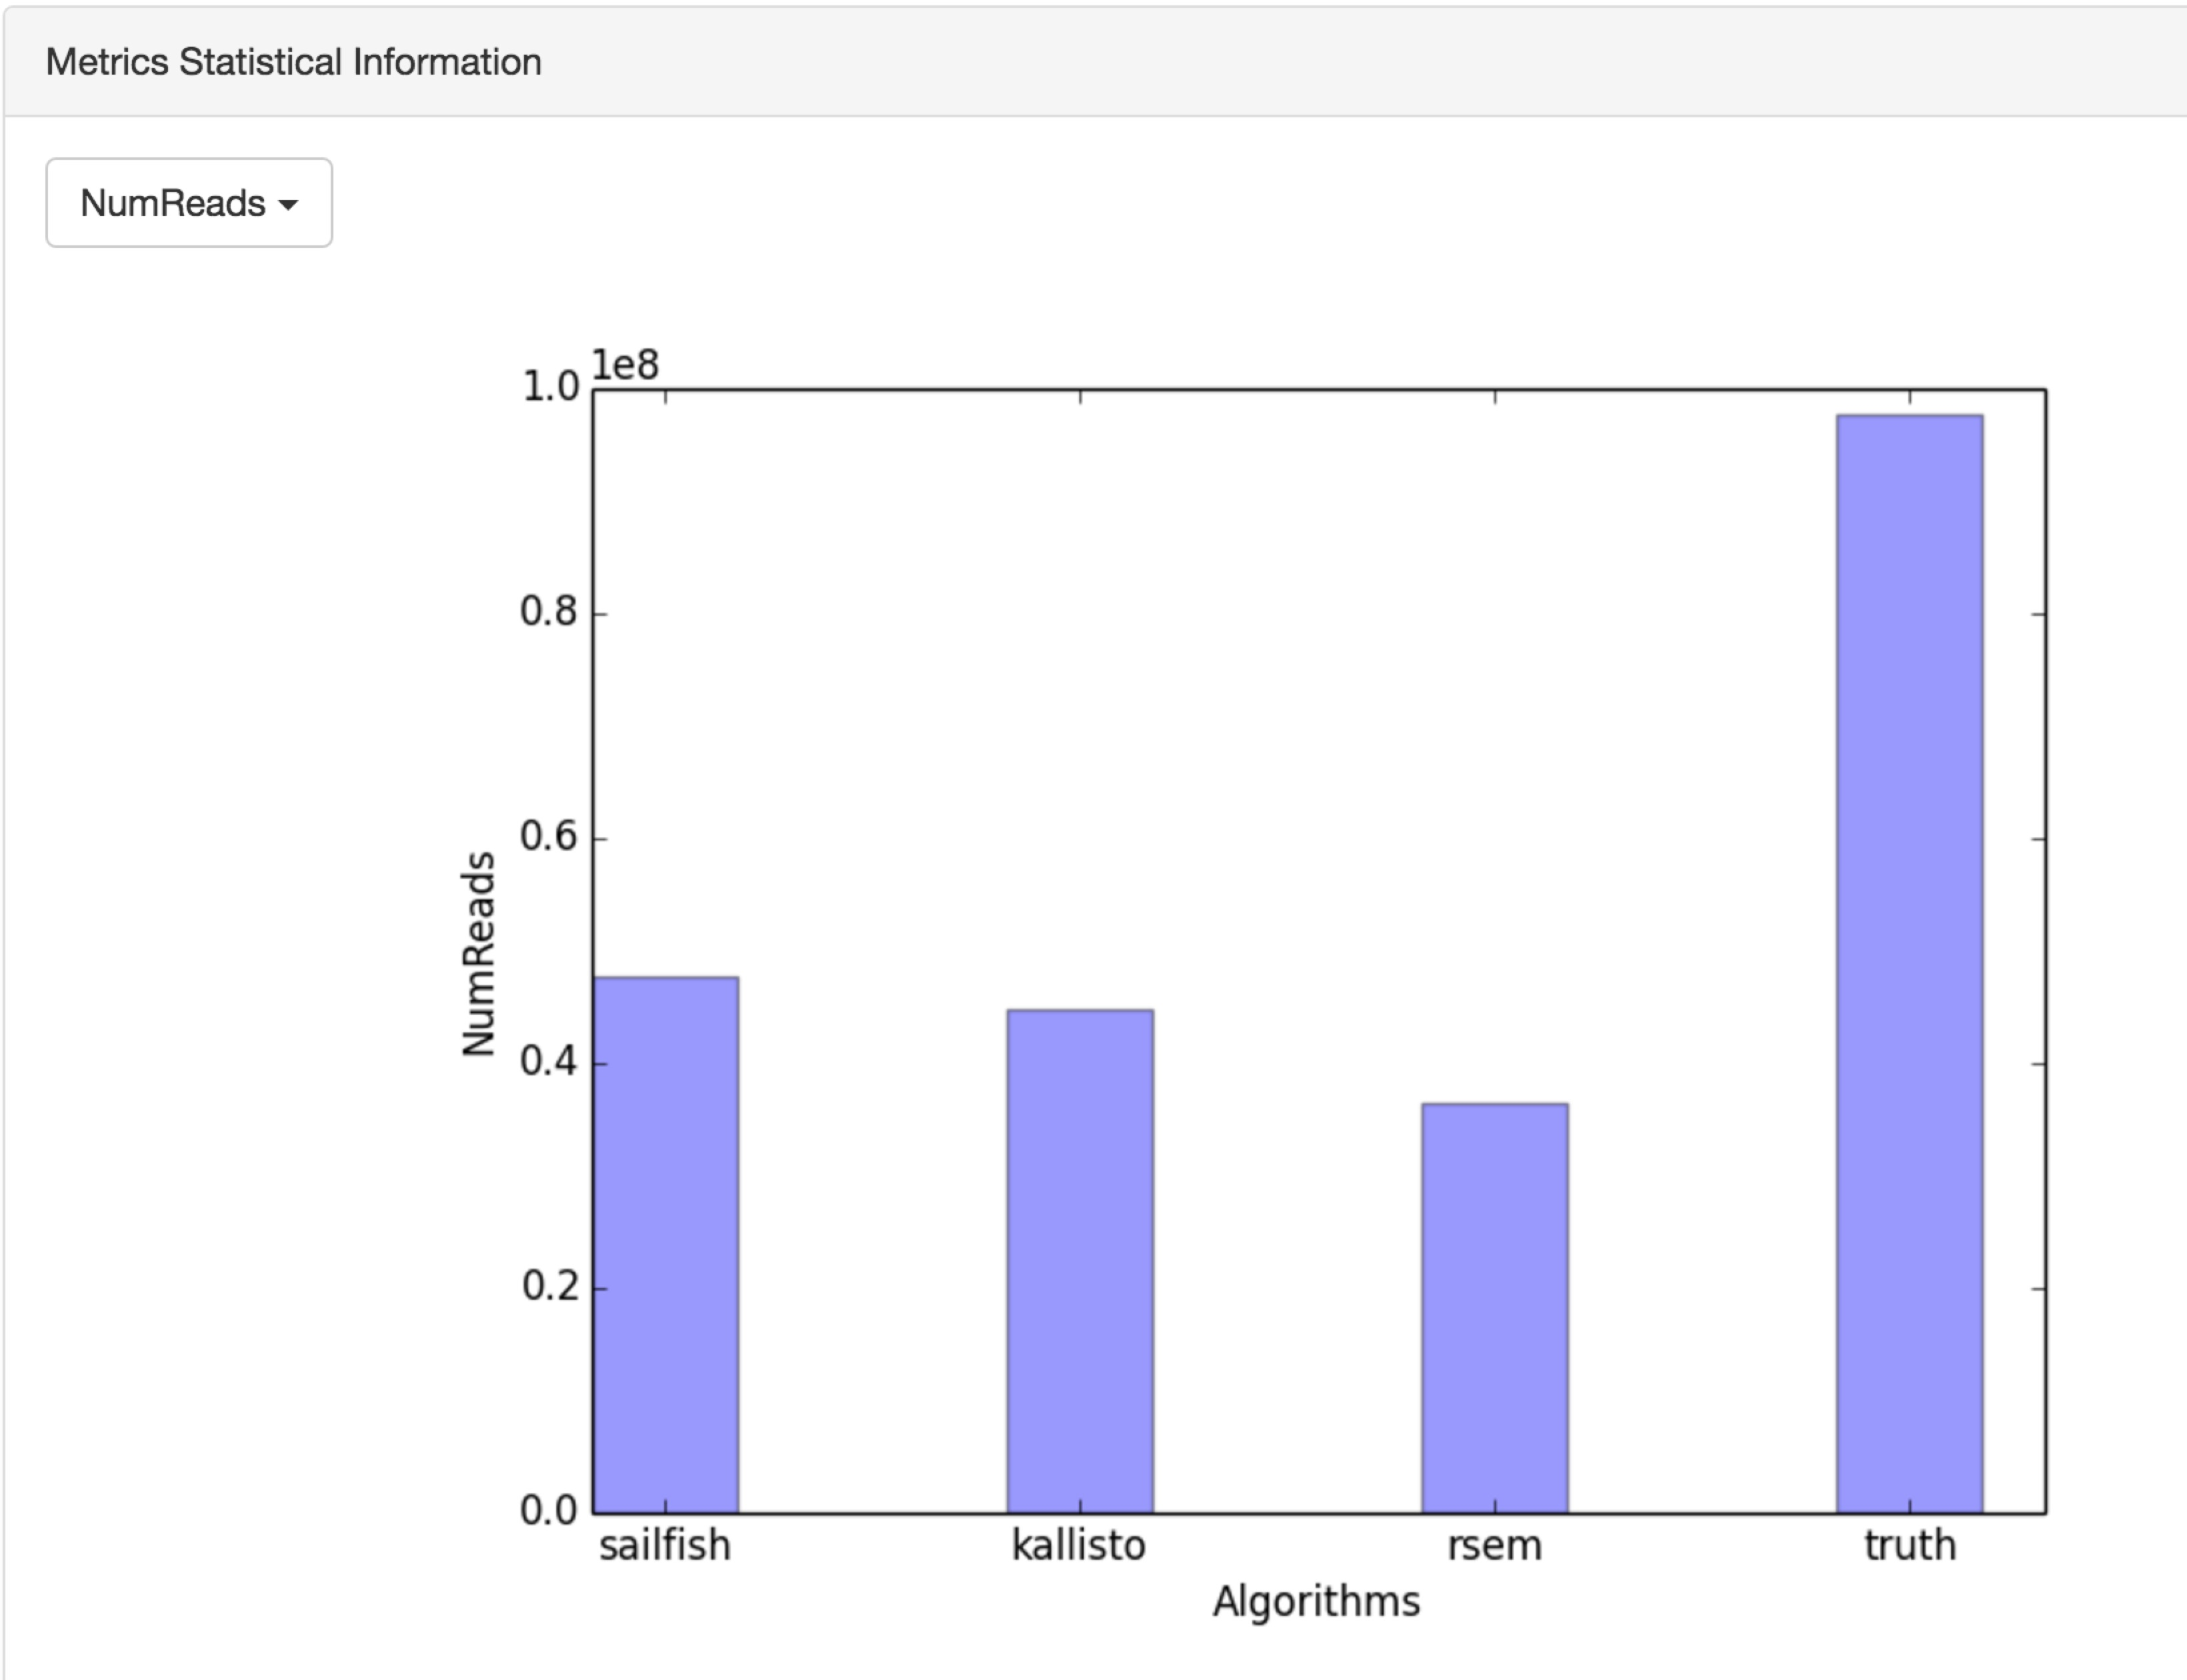
\includegraphics[width=.6\linewidth]{./fig/barchar_numreads.jpg}
 \caption{Bar Chart - NumReads}
  \label{fig:barchart_numreads}
\end{figure}

\subsection {Scatter Plot for a Single Algorithm}
For a single algorithm, we support the scatter plot about any two values such as transcript GC content versus abundance estimates. To plot a scatter plot, the user could go to the scatter plot for single algorithm page, choose an algorithm and the x-axis feature and the y-axis feature. With such a plot, every node on the scatter plot is one transcript and the coordinate is the chosen value pairs and as one example, the scatter plot for sailfish is showed in figure \ref{fig:single_algo_sailfish}. \\
For an interactive mode, you could move the mouse to a node you want to view and the information would automatically showed as in figure \ref{fig:interactive_single_algo_sailfish}.

\begin{figure}[ht]
\centering
\begin{minipage}[b]{0.47\linewidth}
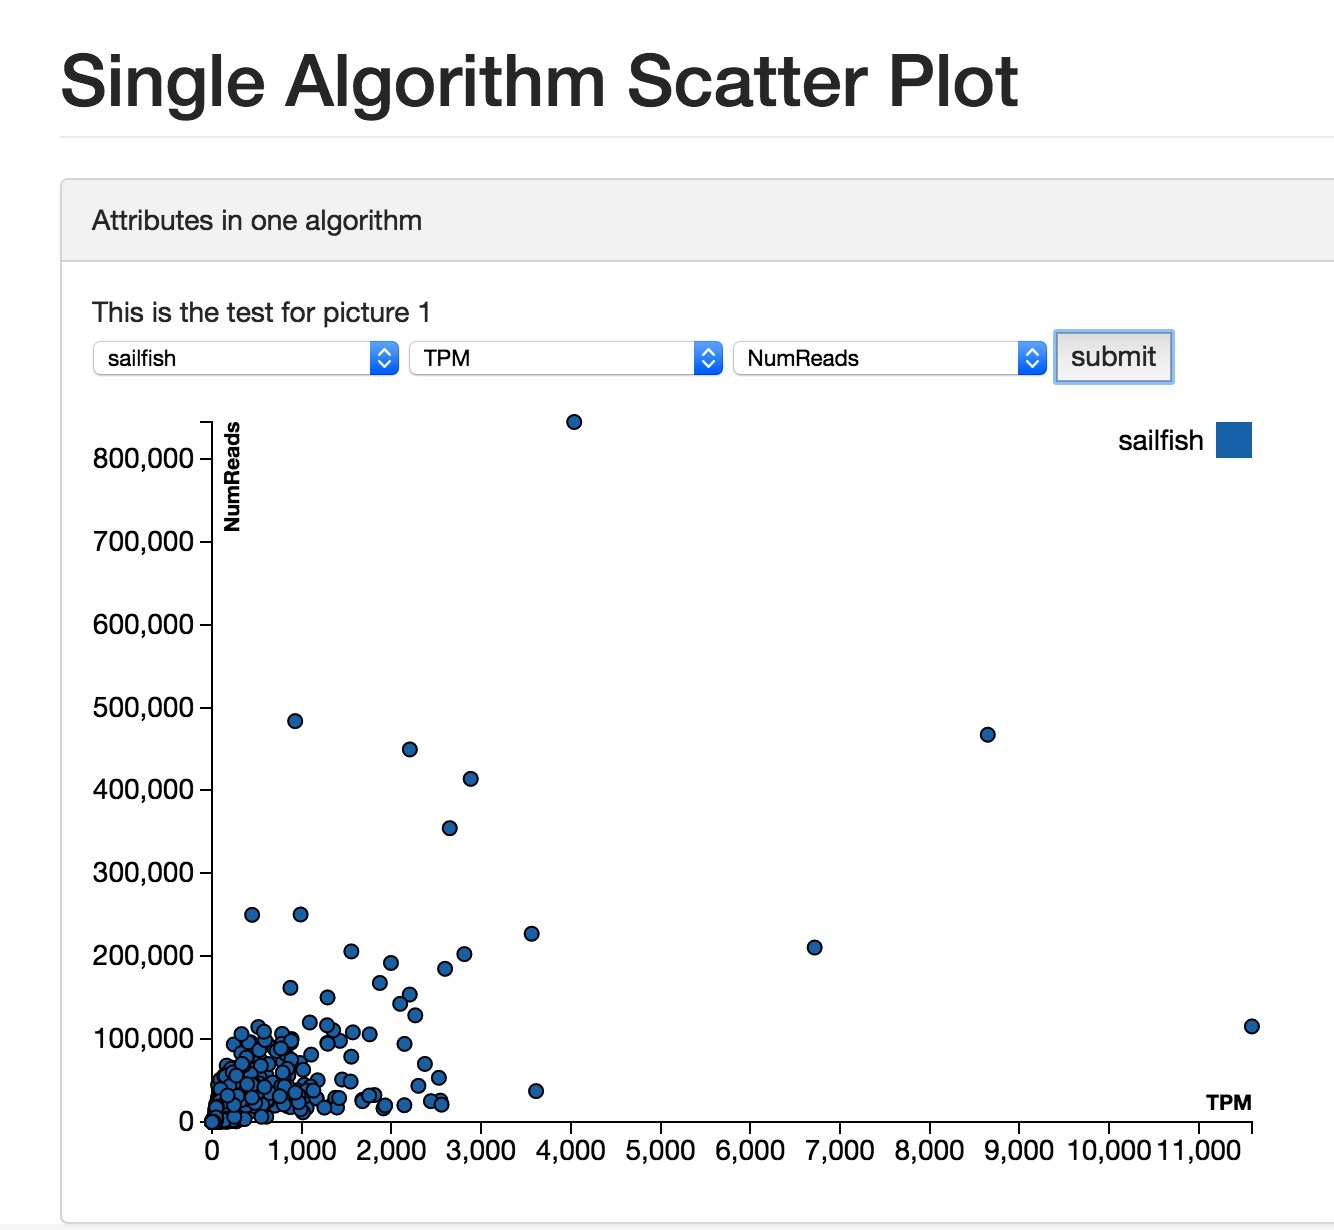
\includegraphics[width=1.0\textwidth]{./fig/single_algo_sailfish.jpg}
\caption{Sailfish - NumReads}
\label{fig:single_algo_sailfish}
\end{minipage}
\quad
\begin{minipage}[b]{0.47\linewidth}
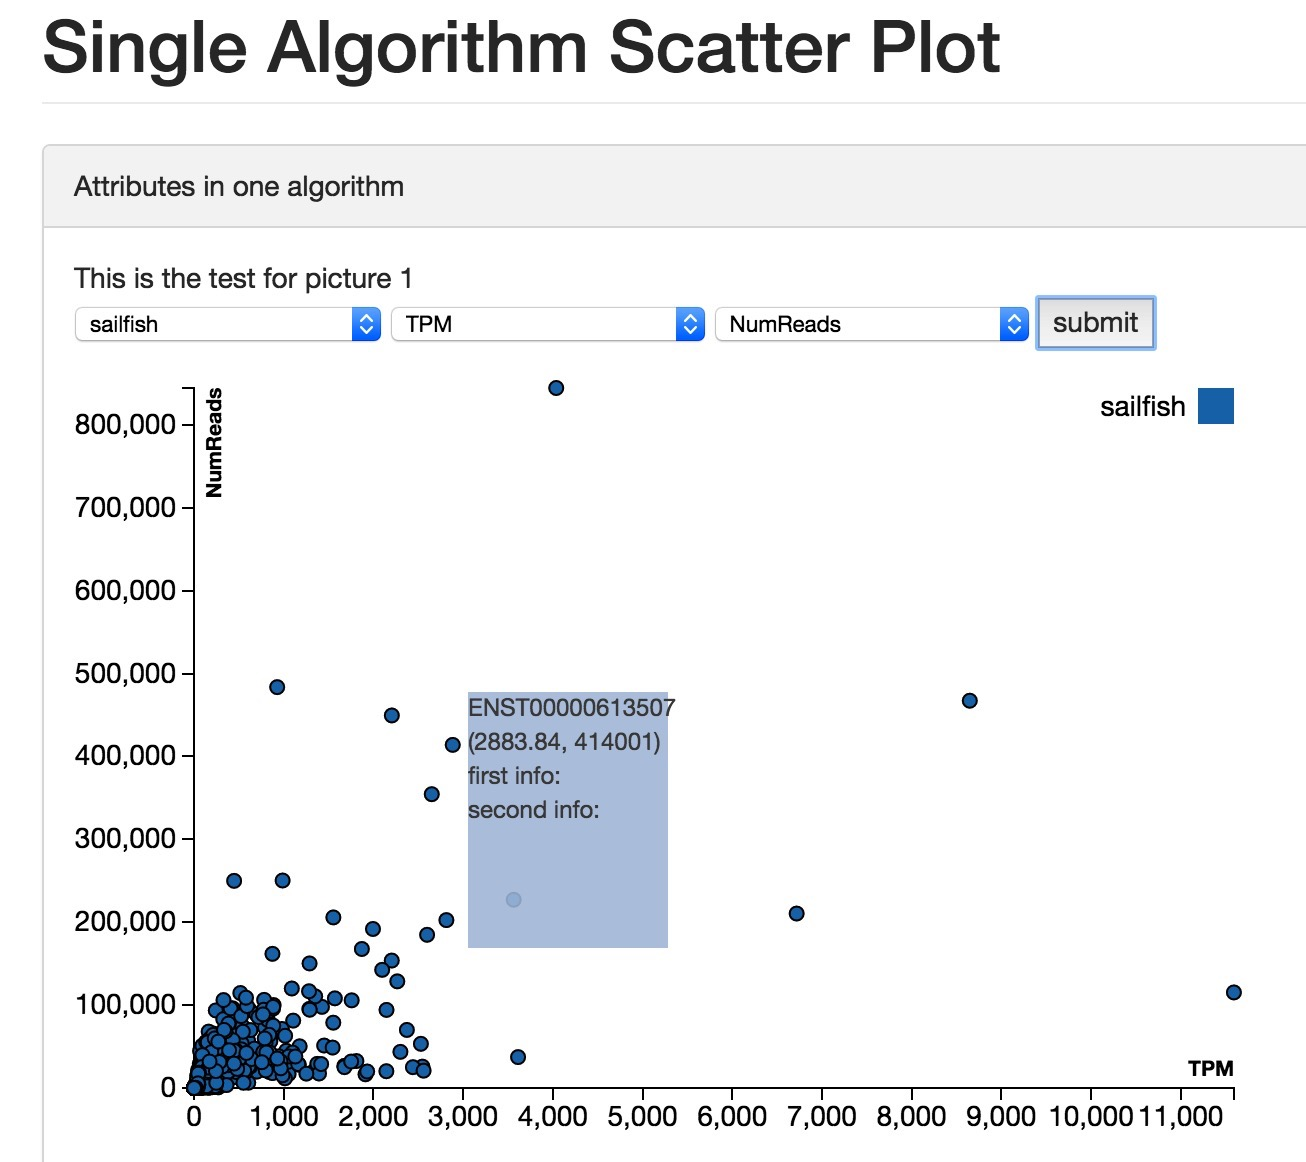
\includegraphics[width=1.0\textwidth]{./fig/interactive_single_algo_sailfish.jpg}
\caption{Sailfish - Interactive NumReads}
\label{fig:interactive_single_algo_sailfish}
\end{minipage}
\end{figure}


\subsection {Scatter Plot for two Algorithms on the same metrics}
We could also compare two algorithms based on the same scatter plots. For example, we could compare the distribution between GC Content and Number of Reads for both Sailfish and Kallisto, as showed in figure \ref{fig:two_algo}.



\subsection {Scatter Plot for two Algorithms on the same feature}
The same features from two algorithms are also comparable. For example, Number of Reads for both Sailfish and Kallisto. We expected they are similar if both of them are good algorithms (figure \ref{fig:compare_sk}). And we could also compare it with the ground truth (figure \ref{fig:compare_truth}).

\begin{figure}[ht]
\centering
\begin{minipage}[b]{0.47\linewidth}
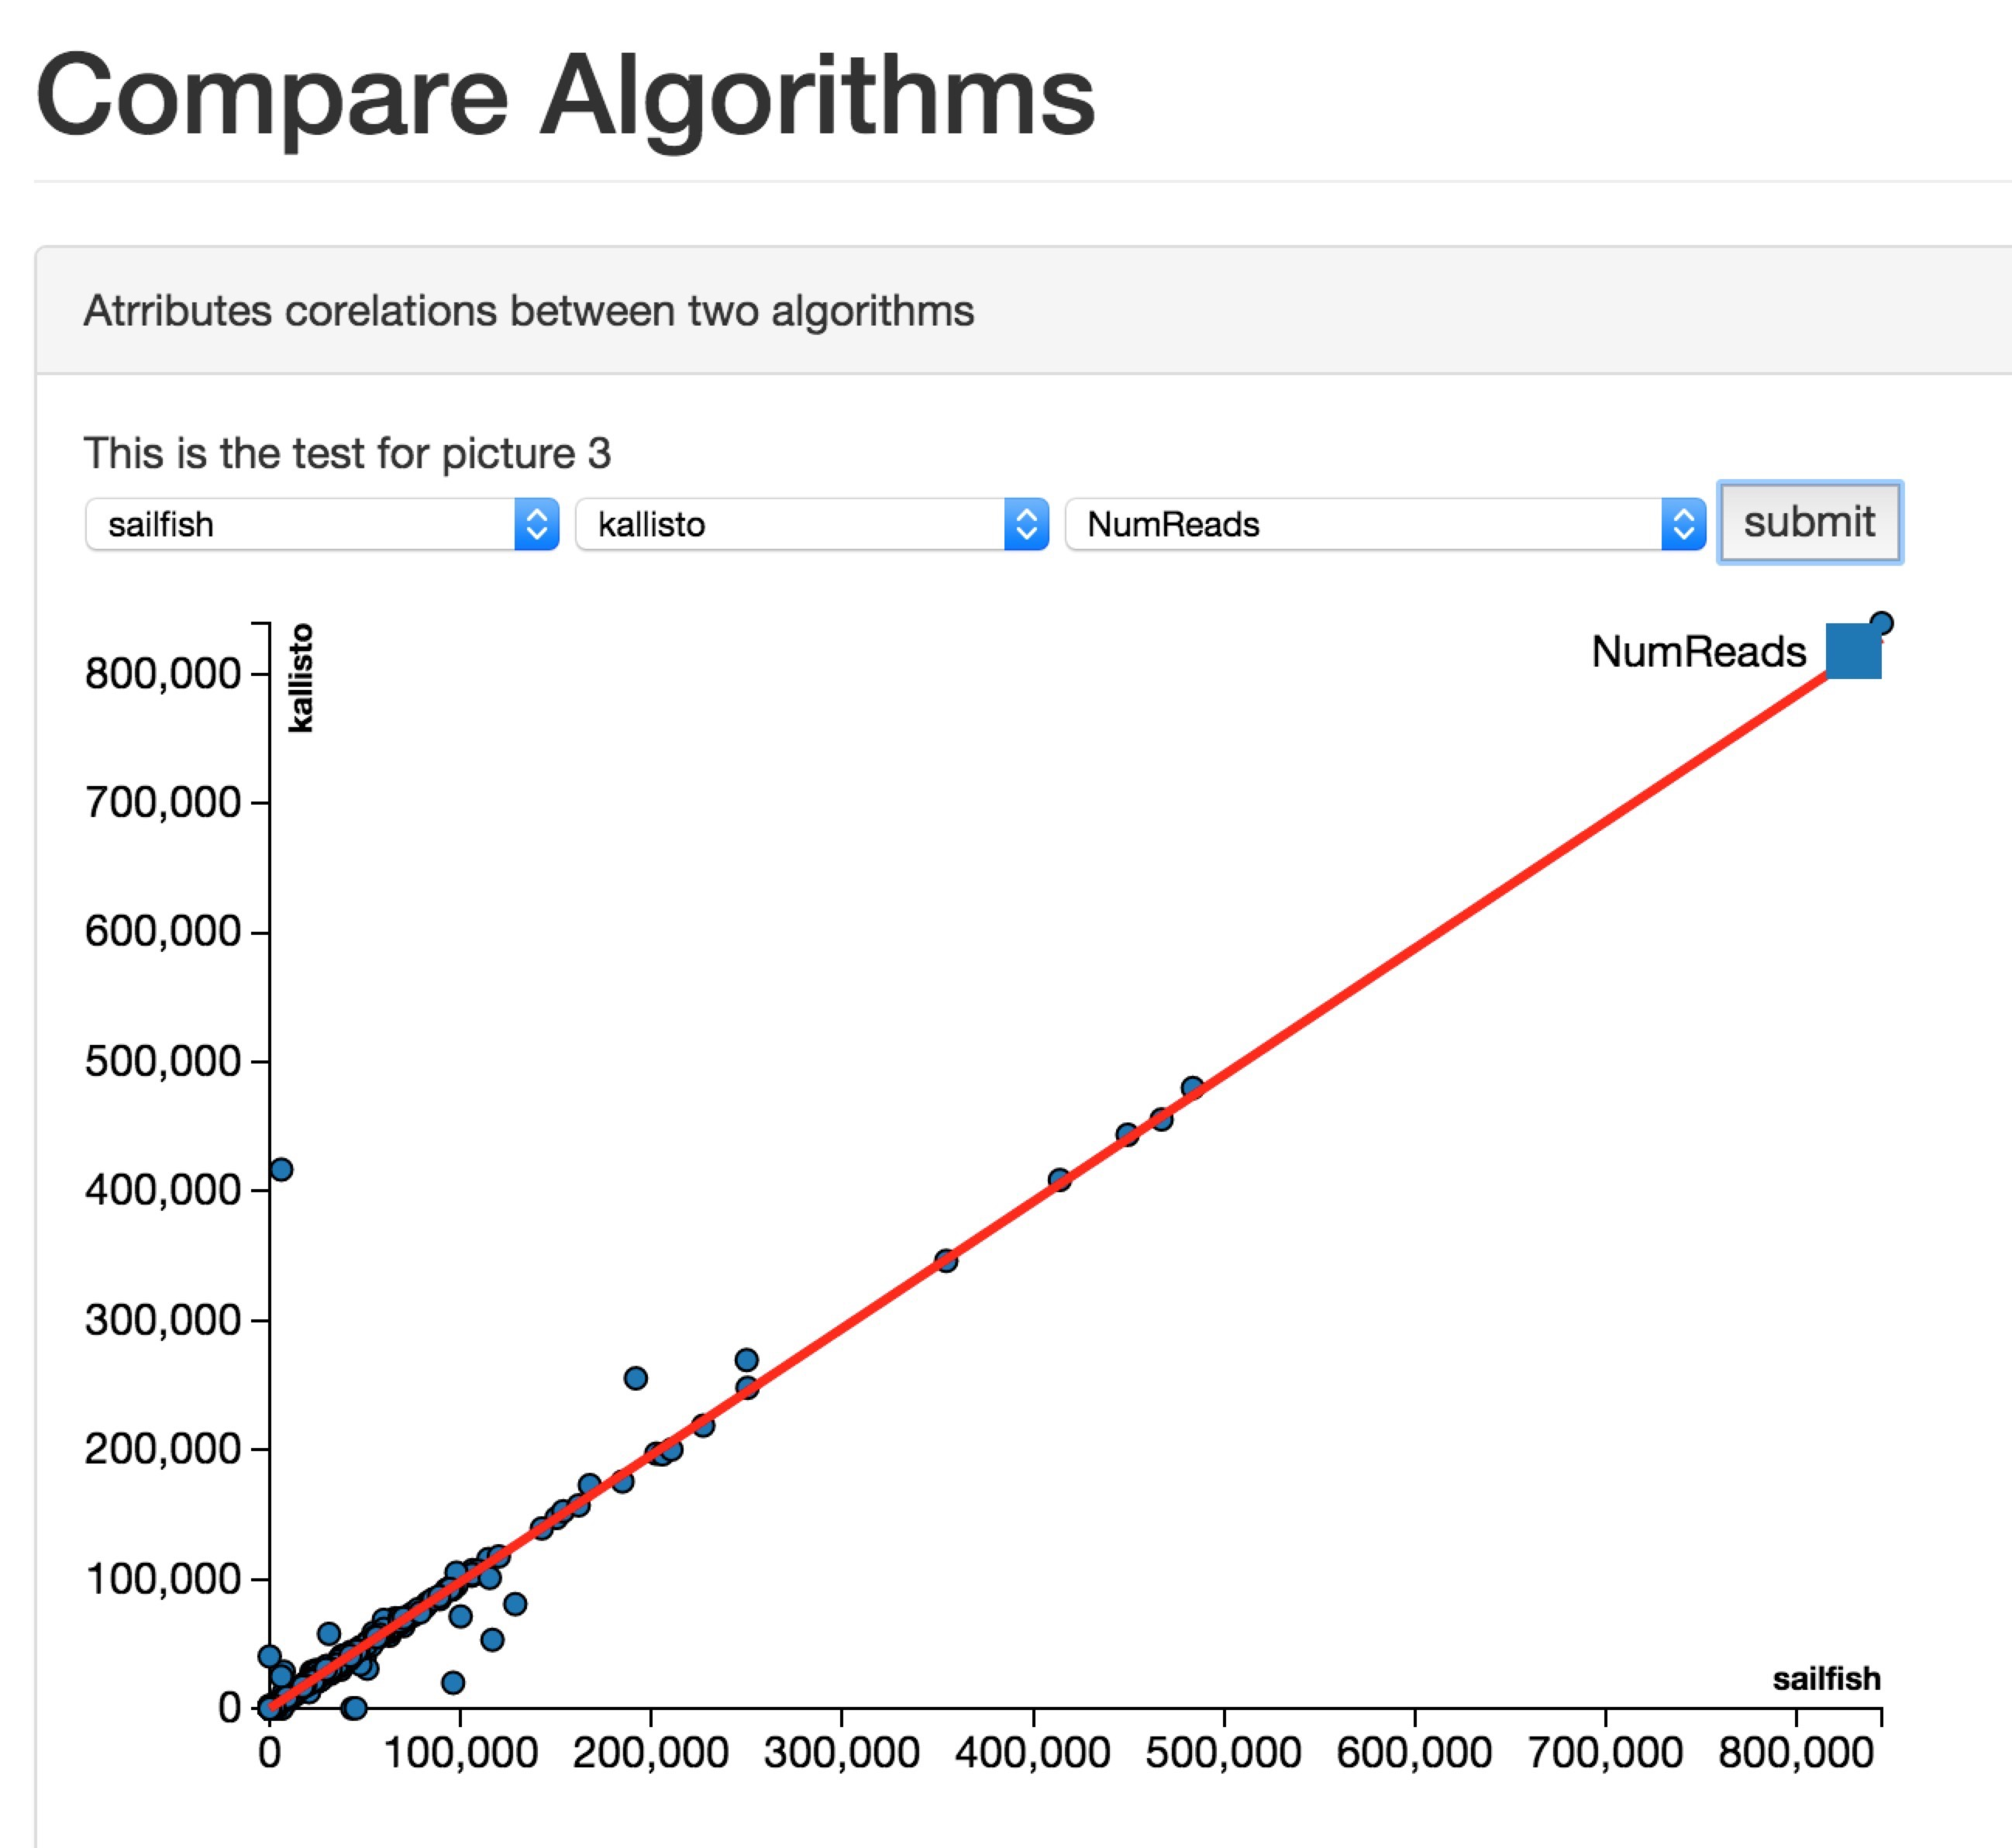
\includegraphics[width=1.0\textwidth]{./fig/compare_sk.jpg}
\caption{Compare NumReads between Sailfish and Kallisto }
\label{fig:compare_sk}
\end{minipage}
\quad
\begin{minipage}[b]{0.47\linewidth}
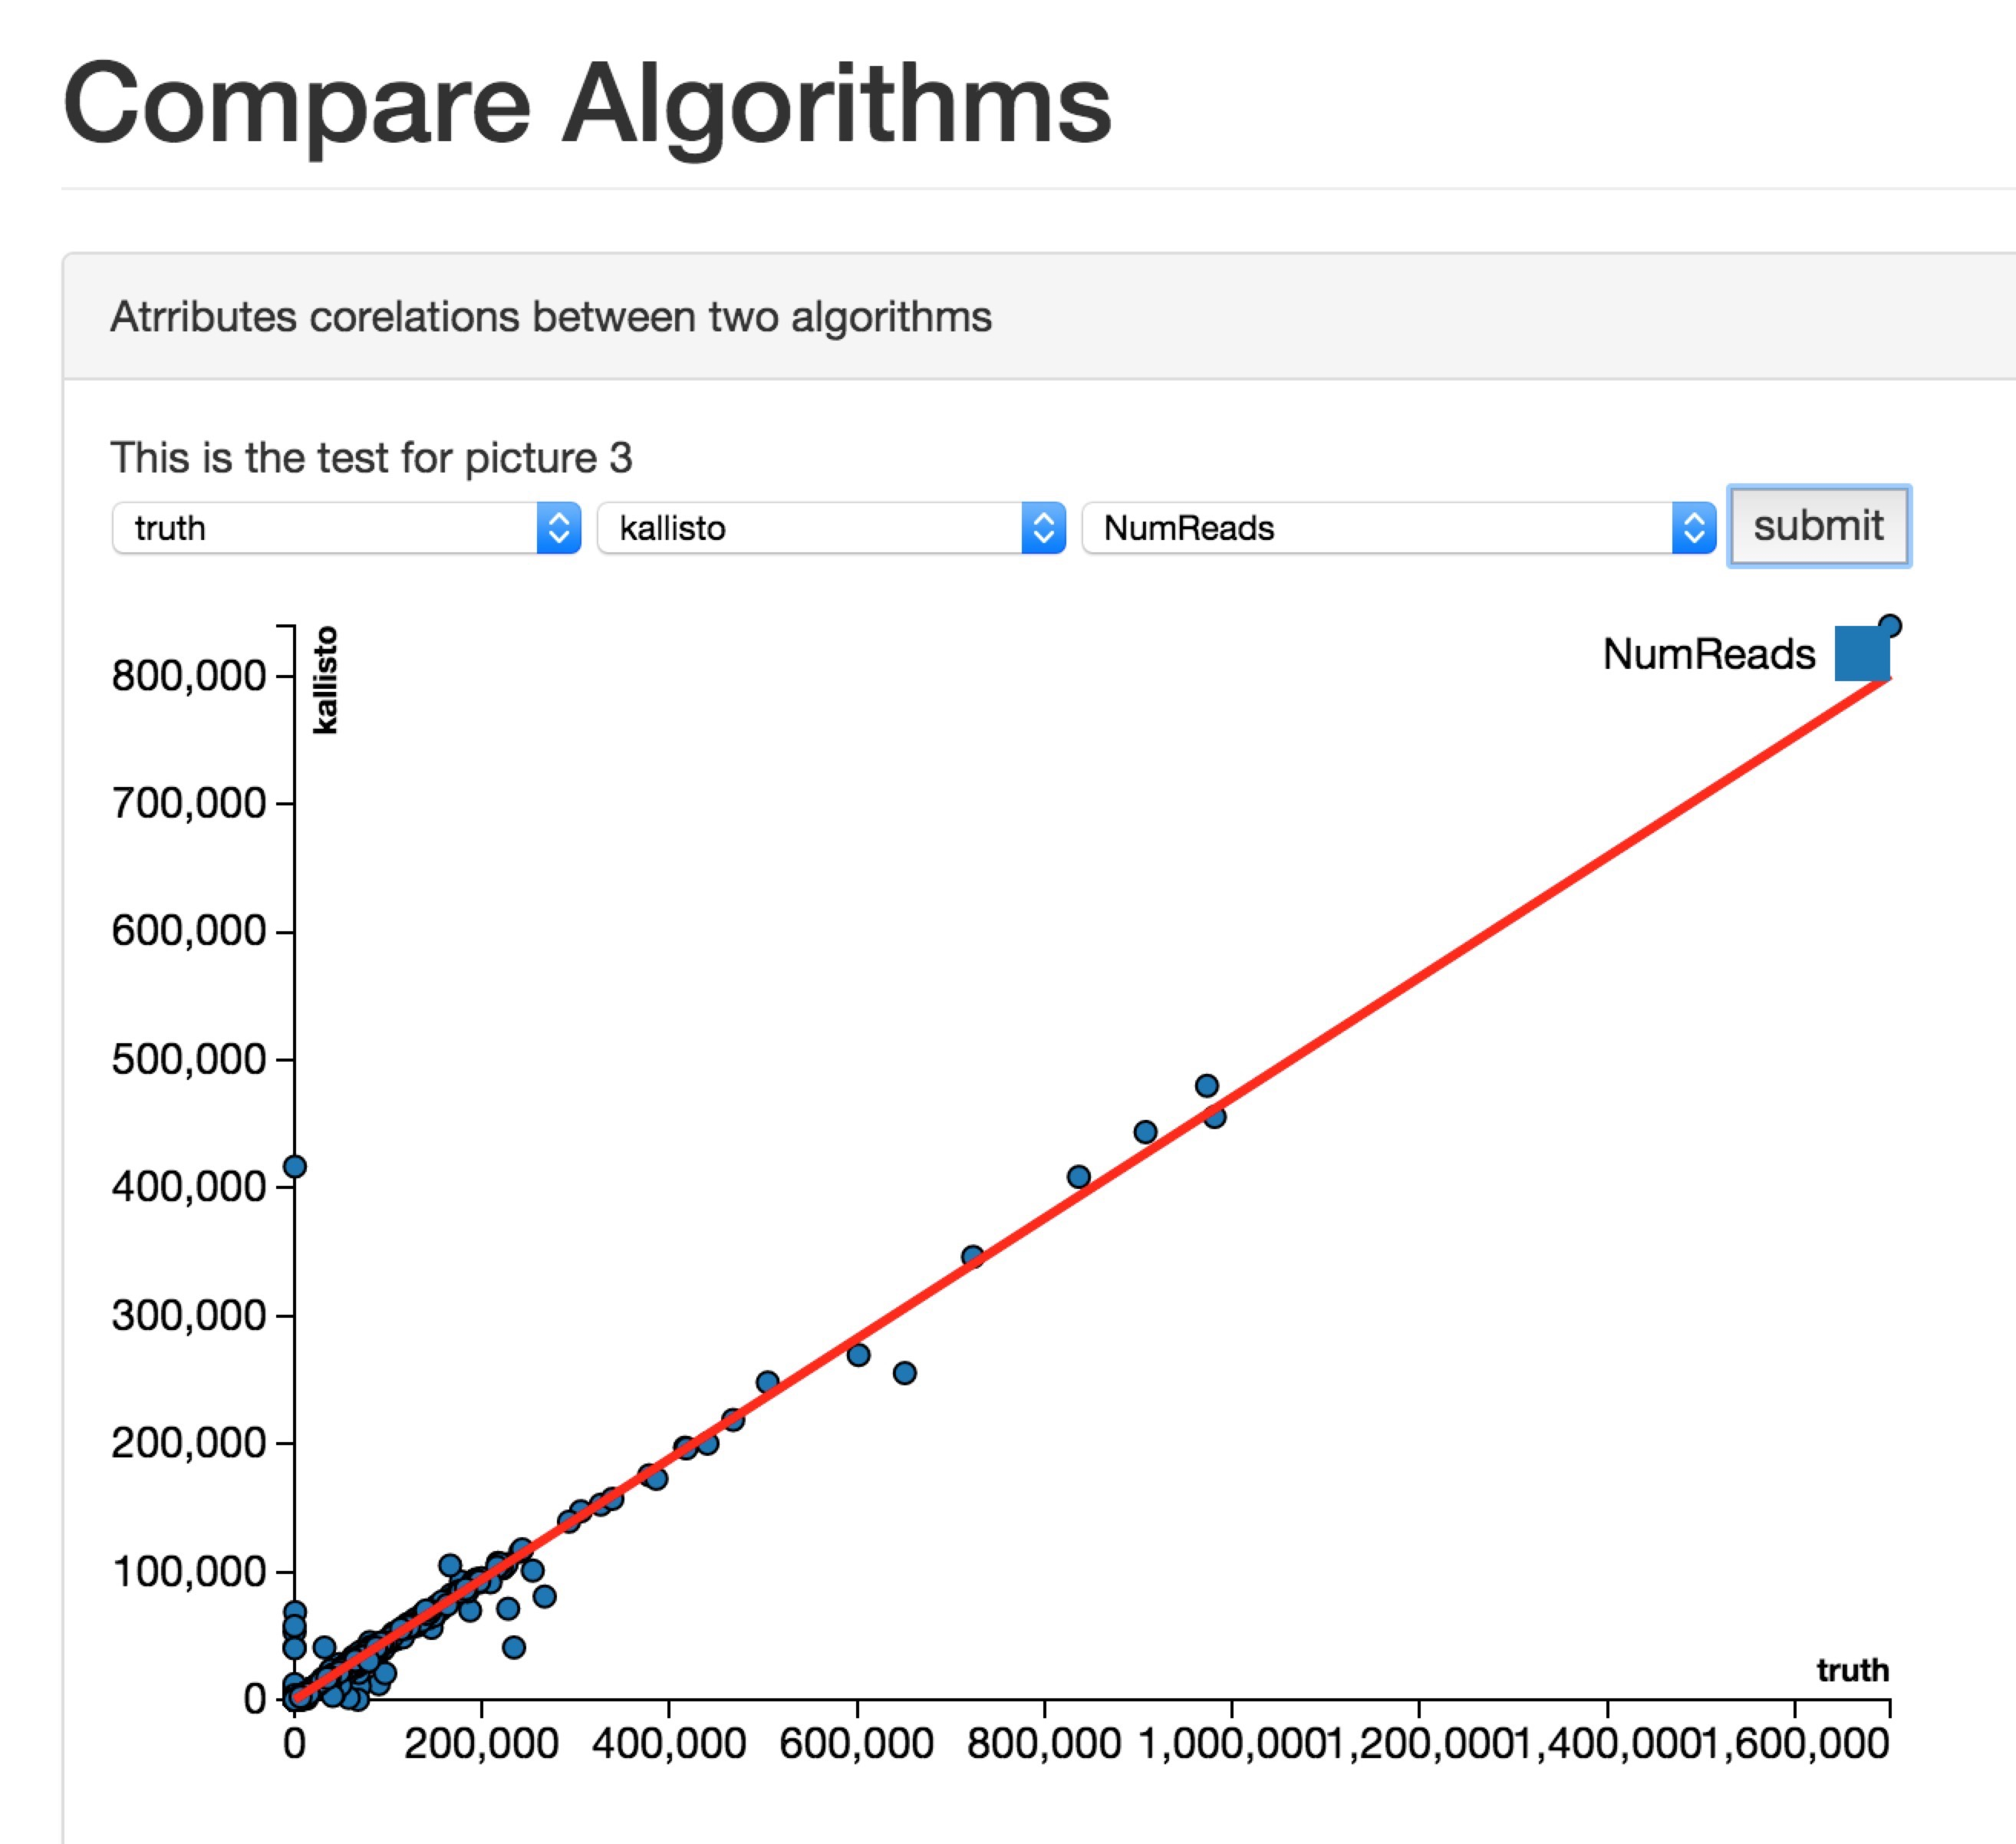
\includegraphics[width=1.0\textwidth]{./fig/compare_truth.jpg}
\caption{Compare NumReads between ground truth and Kallisto  }
\label{fig:compare_truth}
\end{minipage}
\end{figure}

\subsection {Performance Evaluation}
We could also calculate the performance evaluation based on ground truth. The ground truth could be uploaded at upload page showed in figure \ref{fig:metrics}

\begin{figure}[ht]
\centering
\begin{minipage}[b]{0.47\linewidth}
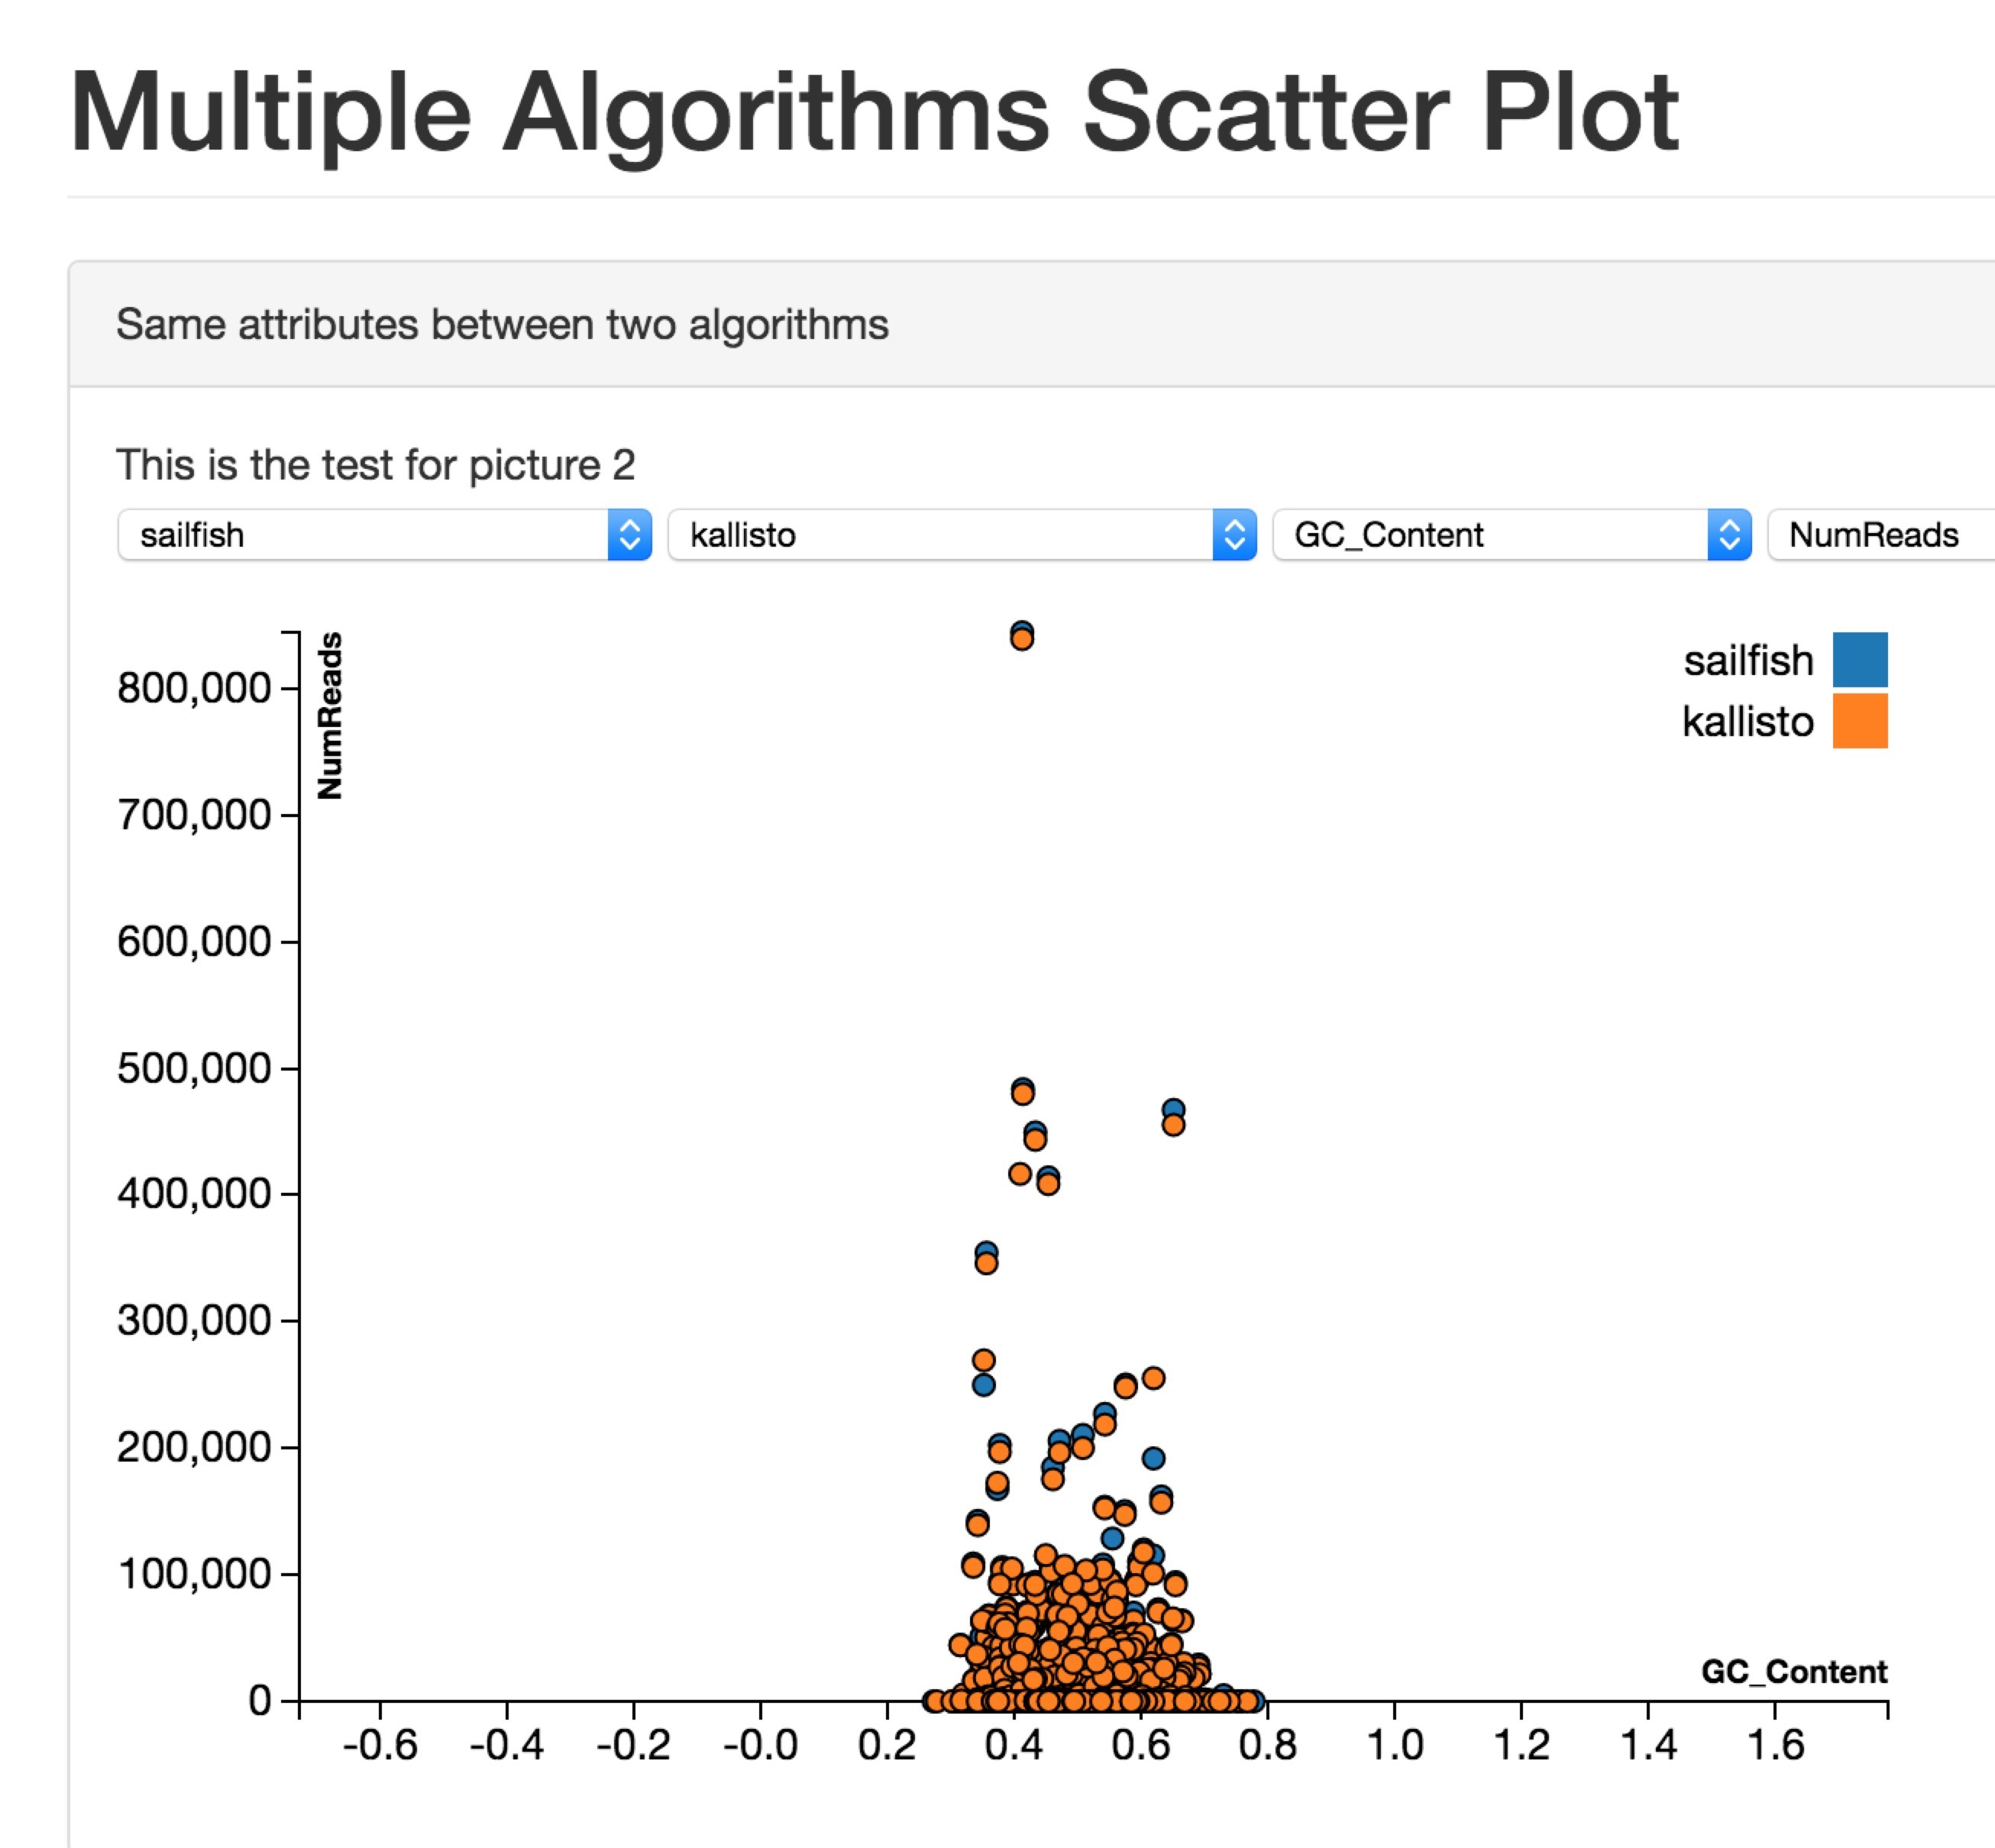
\includegraphics[width=1.0\textwidth]{./fig/two_algo.jpg}
\caption{Sailfish and Kallisto:  GCContent vs  NumReads }
\label{fig:two_algo}
\end{minipage}
\quad
\begin{minipage}[b]{0.47\linewidth}
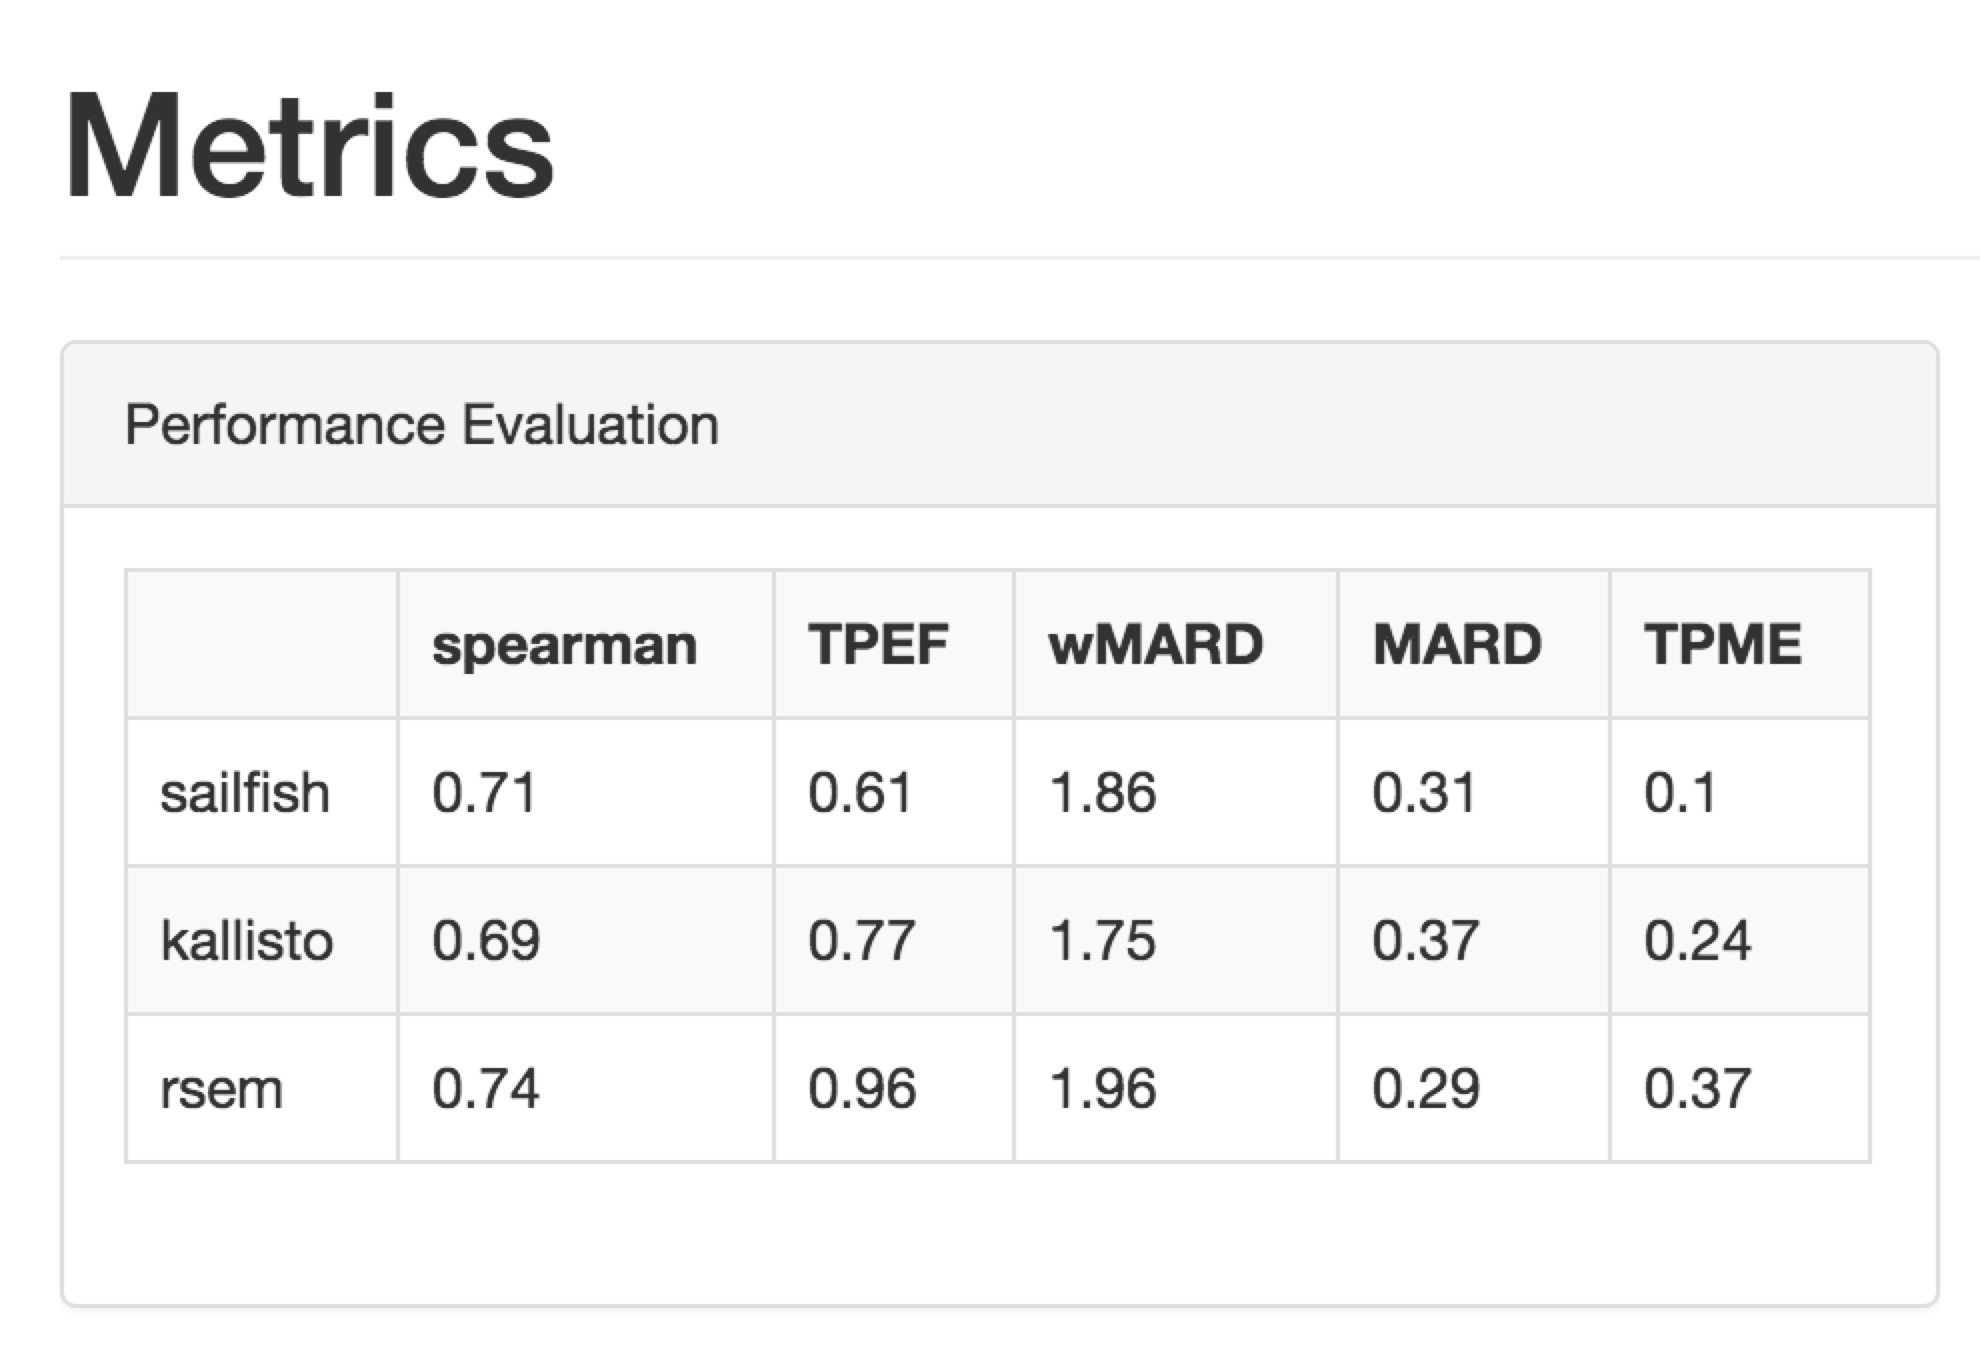
\includegraphics[width=1.0\textwidth]{./fig/metrics.jpg}
  \caption{Performance Evaluation  }
  \label{fig:metrics}
\end{minipage}
\end{figure}

By given the ground truth, we now could calculate the following metrics: Spearman corr., TPEF, TPME, MARD, wMARD \cite{rapmap}.


\section {Extensibility}
\subsection {Upload new data}
Currently the uploading of ground truth is added to re-calculate the performance evaluation results. \\
We also considered the extensibility in our implementation. Currently the result files are directly uploaded to the server side and by upload and rename to the targeted name, call $DataAnalyzor.load_data()$, the server could reload all data to replace the old metrics.
\subsection {Add new algorithm}
To add a new algorithm, one just need to add a related method in $AnalyzorBuilder$  with the corresponding result file, parsing method same as in file $ParsingUtility.py$ and the new algorithm could automatically be supported by the whole framework. \\
At both the front-end and back-end, the algorithms are queried from the $DataAnalyzor$. Once the algorithms and the corresponding methods for reading the data in, the new algorithm and the data would be showed as same as other old features.
\subsection {Add Features to compare}
Currently we support a wide range of comparison: all possible pairs of \\


\section{Acknowledge}
Thanks and regards to Professor Rob Patro's lectures. We were inspired by the algorithms and the vivid examples. \\
Thanks and regards to TA Hirak. He helped us a lot on the project.

% \bibliographystyle{plain}	% (uses file "plain.bst")
% \bibliography{literature}


% \section{References}
\begin{thebibliography}{100} % 100 is a random guess of the total number of
%references
\bibitem{sb_admin_2} "SB Admin 2 - Free Bootstrap Admin Theme." Start Bootstrap. N.p., n.d. Web. 15 Dec. 2015.\\ $<http://startbootstrap.com/template-overviews/sb-admin-2/>$.

\bibitem{d3_scatterplot}"D3 Scatterplot Example." D3 Scatterplot Example. N.p., n.d. Web. 15 Dec. 2015.\\ $<http://bl.ocks.org/weiglemc/6185069>$.

\bibitem{rapmap} Srivastava, Avi, Hirak Sarkar, and Rob Patro. "RapMap: A Rapid, Sensitive and Accurate Tool for Mapping RNA-seq Reads to Transcriptomes." \emph{bioRxiv} (2015): 029652.
\end{thebibliography}

% \input{appendix}

\end{document}
